\sectioncounter{0}
\section{集合的概念与运算}

\subsection{知识梳理}
\myindex{集合} (set) 是一类 (有共性的) 对象的全体, 一般用大写字母表示, 
所考虑的对象称为集合的\myindex{元素} (element), 一般用小写字母表示. 
比如全体整数构成的集合 $A$ 可记为 $\{0,1,-1,2,-2,\cdots\}$,
  \mymarginpar{集合 $\{0,1,-1,2,-2\}$ 不能写成\\ $\{0,\pm1,\pm2\}$.} 
所有大于 1 的数构成的集合 $B$ 可记为 $\{x\mid x>1\}$. 
前一种表示法为\myemph{列举法}, 后一种为\myemph{描述法}. 
有时也用\myemph{韦恩} (Venn) \myemph{图}表示集合.
集合的元素有

(1) \myemph{确定性}: 不能写 $\{\text{比较高的人}\}$;
 
(2) \myemph{互异性}: 不能写 $\{1,1\}$; 

(3) \myemph{无序性}: $\{1,2\}$ 和 $\{2,1\}$ 是同一个集合. 

元素与集合的关系为\myemph{属于} ($\in$) 或\myemph{不属于} ($\notin$),
  \mymarginpar{\myemph{集合的子集}\\
  $\varnothing$ 的子集为 $\varnothing$, 共 $1$ 个;
  $\{a_1\}$ 的子集为 $\varnothing$,$\{a_1\}$, 共 $2$ 个;
  $\{a_1,a_2\}$ 的子集为 $\varnothing$,$\{a_1\}$,$\{a_2\}$,$\{a_1,a_2\}$, 
  共 $4$ 个. 归纳推理可知, $\{a_1,a_2,\cdots,a_n\}$ 的子集有 $2^n$ 个.}
集合与集合的关系为\myemph{包含} ($\subseteq$) 或\myemph{不包含} ($\nsubseteq$).
$A$ 为 $B$ 的子集记作 $A\subseteq B$, 
$A$ 为 $B$ 的真子集记作 $A\subsetneqq B$, 
则 $A\subseteq B$ 且 $A\supseteq B \Leftrightarrow A=B$.
规定空集 ($\varnothing$) 为任何集合的子集, 
并可以推得: 含 $n$ 个元素的集合有 $2^n$ 个子集.

高中数学常考虑的集合是数集和点集. 有的数集也可简写为\myindex{区间} (interval), 
如 

$\{x\mid 1<x<2\}$ 写为 $(1,2)$ (开区间);

$\{x\mid 1\leqslant x\leqslant 2\}$ 写为 $[1,2]$ (闭区间);

$\{x\mid 1< x\leqslant 2\}$ 写为 $(1,2]$ (左开右闭区间).\\
常见数集的简写有: 

$\mathbb{N}$ (或 {\bfseries N}) 表示自然数集; 
$\mathbb{Z}$ (或 {\bfseries Z}) 表示整数集; 

$\mathbb{Q}$ (或 {\bfseries Q}) 表示有理数集;
$\mathbb{R}$ (或 {\bfseries R}) 表示实数集, 等等.\\
常见的点集有: 

中垂线 (到线段两端距离相等的点的集合);
  \mymarginpar{角平分线如何用点集的语言描述?}

圆 (到定点的距离等于定长的点的集合);

椭圆 (到两个定点距离之和为定值的点的集合), 等等.

集合的运算有\myemph{交} ($\cap$, 取公共元素), 
\myemph{并} ($\cup$, 取所有元素),
\myemph{补} ($\complement_U$, 取所有不在原集合但在全集 $U$ 中的元素).
\mymarginpar{用韦恩图表示如下:\\[.2cm]
  \centerline{
  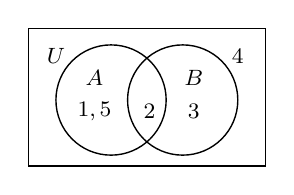
\begin{tikzpicture}[scale=0.7]
    \draw [line width=0.5pt] (0,0) rectangle (4.3,2.5);
    \draw [line width=0.5pt] (1.5,1.2) circle (1cm);
    \draw [line width=0.5pt] (2.8,1.2) circle (1cm);
    \begin{footnotesize}
    \draw (0.5,2) node {$U$};
    \draw (3.8,2) node {$4$};
    \draw (1.2,1.6) node {$A$};
    \draw (1.2,1) node {$1,5$};
    \draw (3,1.6) node {$B$};
    \draw (3,1) node {$3$};
    \draw (2.2,1) node {$2$};
    \end{footnotesize}
  \end{tikzpicture}}}
例如, 设全集为 $U=\{1,2,3,4,5\}$, $A=\{1,2,5\}$, $B=\{2,3\}$, 则
\[A\cap B=\{2\},\quad A\cup B=\{1,2,3,5\},\quad 
  \complement_U A=\{3,4\}.\]
另外, $A\cap B= A\Leftrightarrow A\subseteq B$, 
$A\cup B= A\Leftrightarrow B\subseteq A$.

\lianxi
\begin{exercise}
  已知集合 $A=\{1,3\}$, $B=\{1,9\}$, 那么 $A\cup B=$\,?
\end{exercise}

\beginsolution
  $A\cup B=\{1,3,9\}$.
\endsolution

\begin{exercise}
  设集合 $P=\{x\mid x>1\}$, $Q=\{x\mid x-2>0\}$, 则 $P\underline{\qquad}Q$
  (填 ``$\subseteq$'' 或 ``$\supseteq$'').
\end{exercise}

\beginsolution
  $Q=\{x\mid x>2\}$, 则 $P\supseteq Q$.
\endsolution

\begin{exercise}
  设集合 $A=\{1,2,3\}$, $B=\{1,x\}$, 若 $A\cup B=A$, 则实数 $x$ 的值为\,?
\end{exercise}

\beginsolution
  \(B\subseteq A\), 则 \(x=2\) 或 \(3\).
\endsolution

\begin{exercise}
  已知集合 $A=\{-1,a\}$, $B=\{2a,b\}$. 若 $A\cap B=\{1\}$, 则 $A\cup B=$\,?
\end{exercise}

\beginsolution
  \(1\in A\) 且 \(1\in B\), 则 \(a=1\), $A=\{-1,1\}$, $B=\{2,b\}$, 
  所以 $b=1$, $B=\{2,1\}$, 故 $A\cup B=\{-1,1,2\}$.
  
  \varexercise 已知集合 $A=\{-1,a\}$, $B=\{2a,a^2\}$. 
  若 $A\cap B=\{-1\}$, 则 $A\cup B=$\,?
  
  此时仍有 $-1\in B\Rightarrow 2a=-1$, $a=-\frac12$, 
  故 $A\cup B=\Big\{-1,-\frac12,\frac14\Big\}$.
\endsolution

\begin{exercise}
  已知集合 $A=\{x\mid -2<x<1\}$, $B=\{x\mid x-a<0\}$. 若 $A\subseteq B$, 
  则实数 $a$ 的取值范围是\,?
\end{exercise}

\beginsolution
  $B=(-\infty,a)$, 则 $a\geqslant 1$ 即 $a\in [1,+\infty)$.
\endsolution

\subsection{要点导学\quad 各个击破}
\subsubsection{集合的运算}
\begin{example}
  (1)  已知全集 $U=\{1,2,3,4\}$, 集合 $A=\{1,2\}$, $B=\{2,3\}$, 
  那么 $\complement_U (A\cup B)=$\,?

  (2) 已知集合 $A=\{x\mid 0< \log_4 x< 1\}$, $B=\{x\mid x\leqslant 2\}$, 
  那么 $A\cap B=$\,?

  (3) 若集合 $A=\{1,2,3\}$, $B=\{1,3,4\}$, 则 $A\cap B$ 的子集个数为\,?
\end{example}

\beginsolution
  (1) $A\cup B=\{1,2,3\}$, $\complement_U (A\cup B)=\{4\}$;
  (2) $A=\{x\mid 1<x<4\}$, $A\cap B=\{x\mid 1<x\leqslant 2\}$;
  (3) $A\cap B= \{1,3\}$, 子集共 $2^2=4$ 个.
\endsolution

\lianxi
\begin{exercise}
  设集合 $A=\{x\mid  0.5<x<2\}$, $B=\{x\mid x^2\leqslant 1\}$, 则 $A\cup B=$\,?
\end{exercise}

\beginsolution
  $B=\{x\mid -1\leqslant x\leqslant 1\}$, $A\cup B=\{x\mid -1\leqslant x<2\}$.
\endsolution

\begin{exercise}
  若全集 $U=\{1,2,3,4\}$, 集合 $M=\{1,2\}$, $N=\{2,3\}$, 
  则 $\complement_U (M\cup N)=$\,?
\end{exercise}

\beginsolution
  $M\cup N= \{1,2,3\}$, $\complement_U (M\cup N)=\{4\}$.
\endsolution

\begin{exercise}
  设全集为 $\mathbb{R}$, 集合 $A=\{u\mid u^2 -9<0\}$, 
  $B=\{x\mid -1<x\leqslant 5\}$, 则 $A\cap (\complement_{\mathbb{R}} B)=$\,?
\end{exercise}

\beginsolution
  $A=\{u\mid -3<u<3\}=(-3,3)$, $\complement_{\mathbb{R}} B=(-\infty,-1]\cup (5,+\infty)$, 则 $A\cap (\complement_{\mathbb{R}} B)= (-3,-1]$.
\endsolution

\subsubsection{集合与集合的关系}
\begin{example}
  设集合 $A=\{x\mid 2\leqslant x\leqslant 6\}$, 
  $B=\{x\mid 2a\leqslant x\leqslant a+3\}$, 若 $B\subseteq A$, 
  求实数 $a$ 的取值范围.
\end{example}

\beginsolution
  (1) 若 $B=\varnothing$, 则 $2a>a+3$, $a>3$;
  (2) 若 $B\neq\varnothing$, 则 $2\leqslant 2a\leqslant a+3\leqslant 6$, 解得 $1\leqslant a\leqslant 3$.
  
  综上知, $a\in [1,+\infty)$.
\endsolution

\lianxi
\begin{exercise}[s]
  设集合 $A=\{1,4,2x\}$, $B=\{1,x^2\}$, 若 $B\subseteq A$, 则实数 $x=$\,?
\end{exercise}

\beginsolution
  (1) 若 $x^2=4$, 则 $x=\pm2$, 检验知 $x=-2$;
  \mymarginpar{此题解出 $x$ 后必须检验是否合题意, 即是否满足集合元素的互异性.}
  (2) 若 $x^2=2x$, 则 $x=0$ 或 $2$, 检验知 $x=0$.
  
  综上知, $x=-2$ 或 $0$.
\endsolution

\subsubsection{课堂评价}
\begin{exercise}
  已知集合 $A=\{1,2,3,4\}$, $B=\{x\mid x<2\}$, 那么 $A\cap B=$\,?
\end{exercise}

\beginsolution
  $A\cap B=\{1\}$.
\endsolution

\begin{exercise}
  设集合 $A=\{1, \sqrt{a}\}$, $B=\{a\}$, 若 $B\subseteq A$, 
  则实数 $a$ 的值为\,?
\end{exercise}

\beginsolution
  (1) 若 $a=1$, 则 $\sqrt{a}=1$, 不合题意;
  (2) 若 $a=\sqrt{a}$, 则 $a=0$ 或 $1$, 检验知 $a=0$.
  
  综上知, $a=0$.
\endsolution

\begin{exercise}
  已知集合 $A=\{0,1,2\}$, 那么集合 $B=\{x-y\mid x,y\in A\}$ 中元素的个数是\,?
\end{exercise}

\beginsolution
  $B=\{-2,-1,0,1,2\}$, 共 $5$ 个元素.
  
  \varexercise $A$ 不变, $B$ 改为 $B=\{x+y\mid x,y\in A\}$.
  
  此时 $B=\{0,1,2,3,4\}$, 共 $5$ 个元素.
  
  \varexercise $A=\{0,1,2,\cdots,n\}$, 其中 $n$ 为正整数, $B=\{x-y\mid x,y\in A\}$, $C=\{x+y\mid x,y\in A\}$.
  
  此时 $B=\{-n,-(n-1),\cdots,0,\cdots,n-1,n\}$, 
  $C=\{0,1,2,\cdots,2n\}$, 共 $2n+1$ 个元素.
  
  \varexercise $A=\{(x,y)\mid x,y=0,1,2\}$, $B=\{(x_1+x_2,y_1+y_2)\mid (x_1,y_1), (x_2,y_2)\in A\}$.
  
  此时 $B=\{(x,y)\mid x,y=0,1,2,3,4\}$, 共 $25$ 个元素.
  
  \varexercise $A=\{(x,y)\mid x,y=0,1,2,\cdots,n\}$, 其中 $n$ 为正整数, $B$ 同上.
  
  此时 $B=\{(x,y)\mid x,y=0,1,2,\cdots,2n,2n+1\}$, 共 $(2n+1)^2$ 个元素.
\endsolution

\subsection{课后练习}
\begin{exercise}
  设集合 $A=\{-2,0,2\}$, $B=\{x\mid x^2-x-2=0\}$, 则 $A\cap B=$\,?
\end{exercise}

\beginsolution
  $B=\{-1,2\}$, $A\cap B=\{2\}$.
  
  \varexercise $A$ 不变, $B=\{x\mid x^2-x-2\leqslant 0\}$, 则 $B=[-1,2]$, $A\cap B=\{0,2\}$.
  
  \varexercise $A$ 不变, $B=\{x\mid x^2-x-2> 0\}$, 则 $B=(-\infty,-1)\cup(2,+\infty)$, $A\cap B=\{-2\}$.
\endsolution

\begin{exercise}
  设集合 $A=\{x\mid x^2-2x<0\}$, $B=\{x\mid 1\leqslant x\leqslant 4\}$, 
  则 $A\cap B=$\,?
\end{exercise}

\beginsolution
  $A=\{0,2\}$, $A\cap B=[1,2)$.
\endsolution

\begin{exercise}
  设集合 $A=\{1,2,3\}$, $B=\{4,5\}$, $M=\{x\mid x=a+b,a\in A,b\in B\}$, 
  则 $M$ 中的元素个数为\,?
\end{exercise}

\beginsolution
  $M=\{5,6,7,8\}$, 共 $4$ 个元素.
  
  \varexercise 若 $A=\{(x,y)\mid |x|+|y|\leqslant 3, x,y\in\mathbb{Z}\}$, $B=\{(x,y)\mid x,y=0,1\}$, $M=\{(x_1+x_2,y_1+y_2)\mid (x_1,y_1)\in A, (x_2,y_2)\in B\}$, 则画图可知, $M$ 共有 $40$ 个元素.
\endsolution

\begin{exercise}
  若集合 $A=\{x\mid y=\sqrt{x-1}\}$, $B=\{y\mid y=x^2 +2\}$, 则 $A\cap B=$\,?
\end{exercise}

\beginsolution
  $A=[1,+\infty)$, $B=[2,+\infty)$, 则 $A\cap B=[2,+\infty)$.
\endsolution

\begin{exercise}
  已知全集为 $\mathbb{R}$, 集合 $A=\Bigl\{x\Bigm|\Big(\dfrac12\Big)^x\leqslant 1\Bigr\}$,
  $B=\{x\mid x^2-6x+8\leqslant 0\}$, 那么 $A\cap (\complement_{\mathbb{R}} B)=$\,?
\end{exercise}

\beginsolution
  $A=[0,+\infty)$, $B=[2,4]$, 则 $\complement_{\mathbb{R}} B= (-\infty,2)\cup (4,+\infty)$, $A\cap (\complement_{\mathbb{R}} B)=[0,2)\cup (4,+\infty)$.
\endsolution

\begin{exercise}
  已知集合 $A=\{1,2\}$, $B=\{x\mid 0<x<5, x\in\mathbb{N}\}$, 
  若 $A\subseteq C\subseteq B$, 求满足条件的集合 $C$ 的个数.
\end{exercise}

\beginsolution
  $B=\{1,2,3,4\}$, 则 $C$ 的个数为 $\{3,4\}$ 子集的个数, 即 $2^2=4$ 个.
\endsolution

\begin{exercise}
  已知集合 $A=\{x\mid x^2-px+15=0\}$, $B=\{x\mid x^2-ax-b=0\}$, 
  $A\cup B=\{2,3,5\}$, $A\cap B=\{3\}$, 求 $p$, $a$, $b$ 的值.
\end{exercise}

\beginsolution
  由 $3\in A$ 知 $p=8$, $A=\{3,5\}$, 所以 $B=\{2,3\}$. 由韦达定理, $a=5$, $-b=6$ 即 $b=-6$.
\endsolution

\begin{exercise}
  已知集合 $A=\{x\mid 1<x<3\}$, 集合 $B=\{x\mid 2m<x<1-m\}$.

  (1) 当 $m=-1$ 时, 求 $A\cup B$;
  
  (2) 若 $A\subseteq B$, 求实数 $m$ 的取值范围;

  (3) 若 $A\cap B=\varnothing$, 求实数 $m$ 的取值范围.
\end{exercise}

\beginsolution
  (1) 当 $m=-1$ 时, $B=(-2,2)$, $A\cup B= (-2,3)$.
  
  (2) $A\subseteq B$ 表明 $2m\leqslant 1<3\leqslant 1-m$, 解得 $m\in(-\infty,-2]$.
  
  (3) 若 $B=\varnothing$, 则 $2m\geqslant 1-m$, $m\geqslant \frac13$.
  若 $B\neq\varnothing$, 则 $2m< 1-m\leqslant 1$ 或 $3\leqslant 2m< 1-m$, 即 $0\leqslant m< \frac13$ 或 $m\in\varnothing$.
  
  综上知, $m\in[0,+\infty)$. 
\endsolution

%%%%%%%%%%%%%%%%%%%%%%%%%